\documentclass{atistandalonetask}
\usepackage{atistandard}

\begin{document}
  \begin{atiTask}[
    title = \textsc{Fourier}-Transformationen
  ]
	\begin{atiSubtasks}
	\item Berechnen Sie die \textsc{Fourier}-Transformation der Funktion
	\[
	f(x)=\Theta(x-a)e^{-bx},\quad (b>0)
	\]
	worin $\Theta(x)$ die \textsc{Heaviside}sche Sprungfunktion bedeutet.
	\item Berechnen Sie die \textsc{Fourier}-Transformierte der Funktion
	\[
	f(t)=\begin{cases}
	t^3\quad \text{für}\; 0<t<1\\
	0\quad \text{sonst}
		 \end{cases}
	\]
	durch direkte partielle Integration des Transformationsintegrals.
	\end{atiSubtasks}
  \end{atiTask}
  \begin{atiSolution}
   Lösung folgt
   %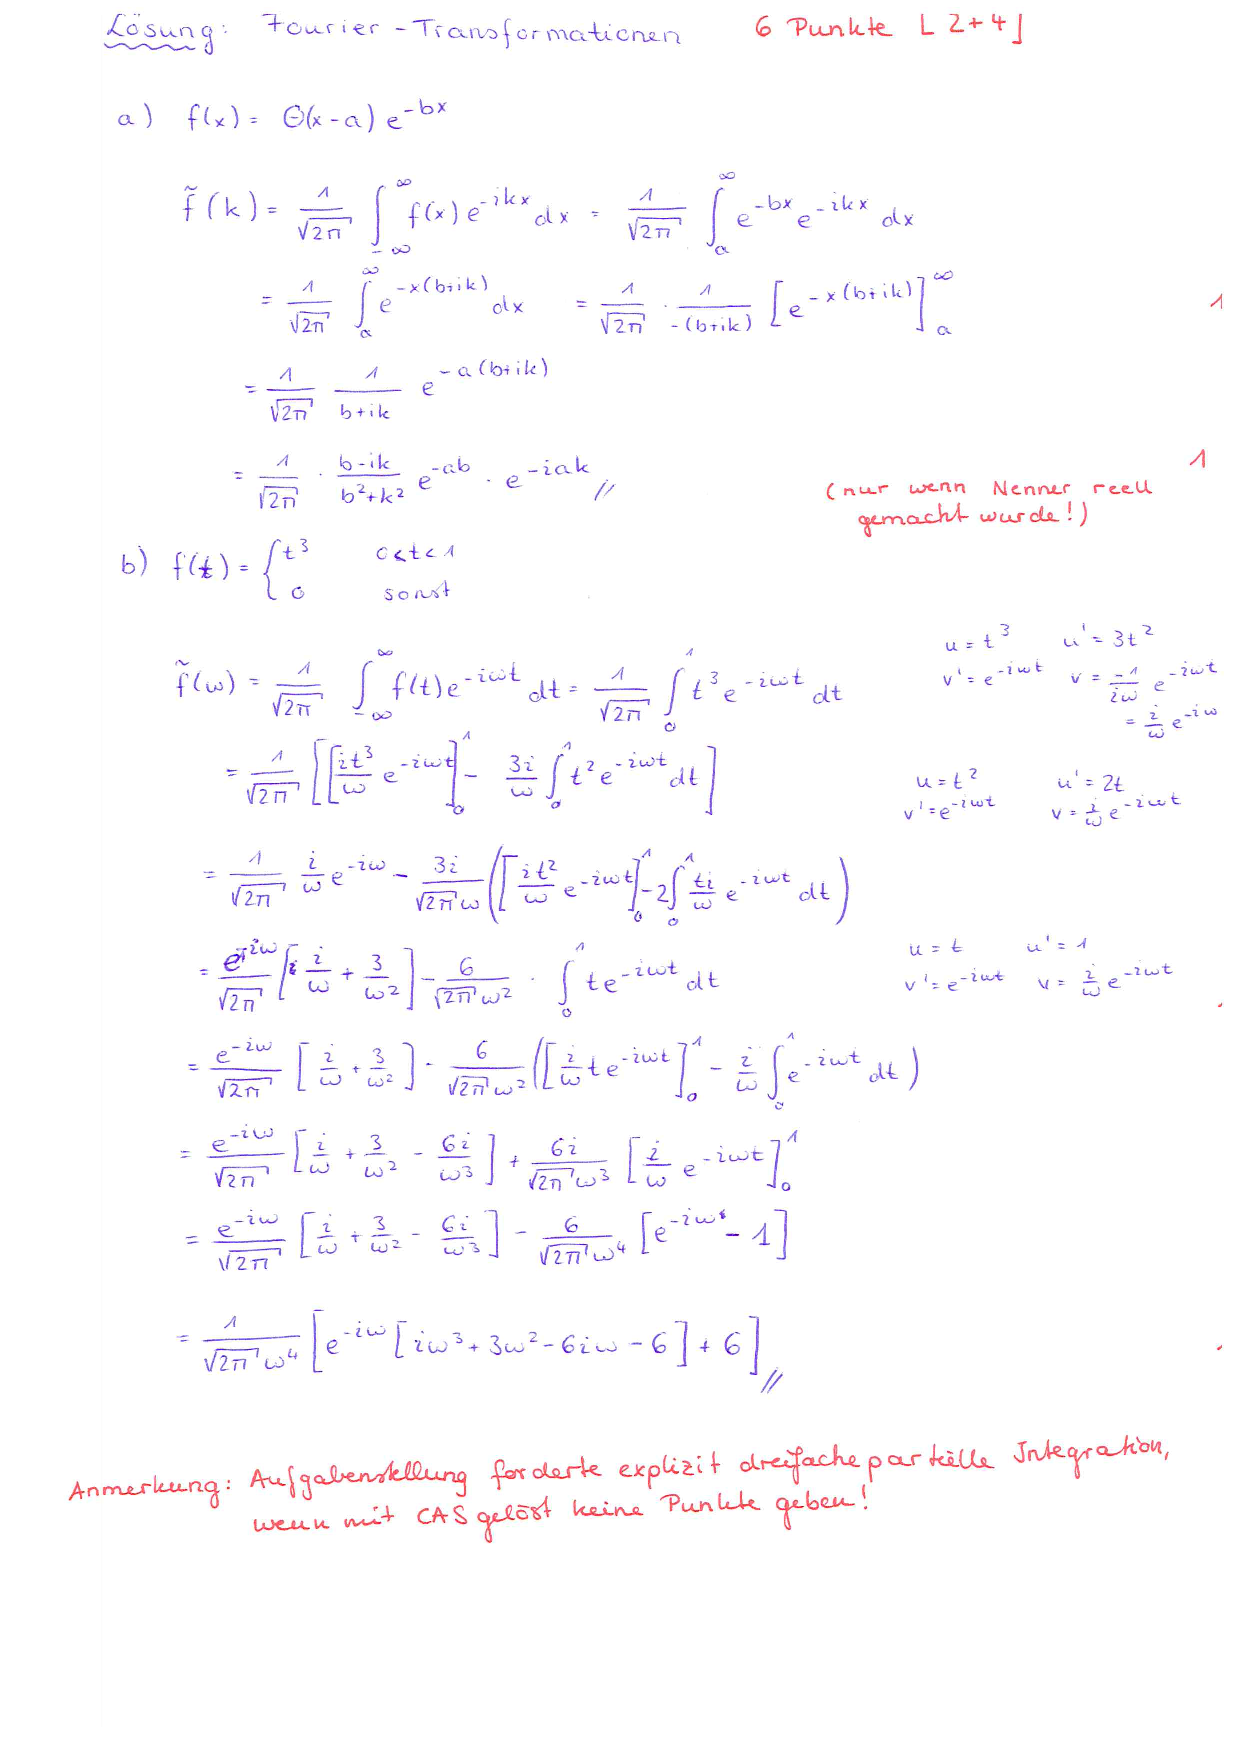
\includepdf[pages=-]{solution-fouriertrafo_i.pdf}
  \end{atiSolution}
\end{document}